\documentclass{article}

%%%%%%%%%%%%%%%%%%%%%%%%%%%%%%%%%%%%%%%%%%%%%%%%%
% Imports
%%%%%%%%%%%%%%%%%%%%%%%%%%%%%%%%%%%%%%%%%%%%%%%%%
%\usepackage[english]{babel}
\usepackage[utf8]{inputenc}
\usepackage[backend=biber,sorting=none,hyperref]{biblatex}
\usepackage{mathtools}
\usepackage{dsfont}
\usepackage{tikz}
\usetikzlibrary{topaths,calc,tikzmark}
\usepackage{algorithm2e}
\usepackage{svg}
\usepackage{listings}
\usepackage{adjustbox}

\svgpath{{svgs/}}

\pagestyle{empty}

\begin{document}

\section{The new algorithms}
The currently fastest algorithm is pretty good.
It's well thought out and quite efficient.
But the algorithm searches a lot of redundant space.
Some colorings have to have the same validity as others and search them as many times as there are duplicates ($r!$) is a waste.
The key insight is that we can end some searches earlier if we know we eventually reach a coloring with equivalent validity.


There are some different kinds of colorings that I've decided to group in a very specific way.
We always start at the nodes that match the \textit{top-regex}, I call these \textit{top-coloring}.

\subsection{Equivalence classes of colorings}
Consider that we use the colors $a, b, c, d \dots$. We order them alphabetically which gives us an ordering of the coloring.
The \textit{top-regex} requires all colors and exactly one of each color in ``rising`` order with the first colors spread between them.
All colors also have to be present, so we only allow surjective colorings.
\\[1em]
\textit{top-regex}: $aa*ba*ca*\dots$ \hspace{1em} \textit{e.g.}: $abc$, $abaca$, $aabaacaa$
\\[1em]
There are also equivalence classes, where colorings which have to be valid at the same time are mapped to.
Consider the colorings $abc$ and $cba$. No matter the edge configuration of the hyper graph, these two colorings have to share validity.
This is because we can rename each color to get the other color -- colorings only care about the internal equality of colors.
We can then send all of these to their representative by renaming the colors. We start from the left and rename all colors, calling
the first color we see $a$, the second $b$ and so on. We can also describe a regex that matches this.
\\[1em]
\textit{eq-regex}: $a[a]*b[ab]*c[abc]*\dots$ \hspace{1em} \textit{e.g.}: $abc$, $ababacaa$, $aabaccab$
\\[1em]
Note specially that if \textit{top-regex} matches, then \textit{eq-regex} also matches. All top-nodes are eq-nodes, \textit{top-reqeg} implies \textbf{eq-regex}.
\textit{eq-regex} matching is a requirement for \textit{top-regex} to match.

% TODO image

\begin{figure}[h!]
  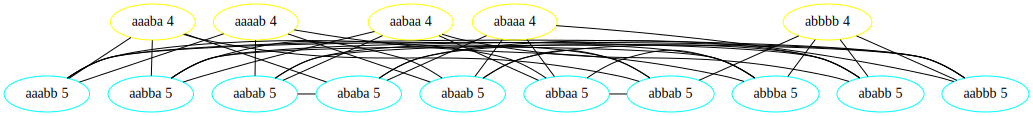
\includegraphics[width=\textwidth]{c_5_2.png}
  \caption{A complete list of all coloring equivalence classes for a hypergraph with 5 nodes and 2 nodes per edge. Edges are between nodes with edit distance 1. \textit{top-node} are drawn above the other nodes. The number of nodes in each class is written after the representative color.}
  \label{fig:eqvClass}
\end{figure}

The Figure \ref{fig:eqvClass} is a super-small example for a toy part of the problem, but I still think it clearly demonstrates the idea for this grouping. Looking at the graphs for coloring of larger problem instances, the visualization quickly becomes unwieldy. 


\subsection{Coloring Categories}
We will also need to reason about what I've decided to call ''coloring categories''. ''coloring categories'' are groupings of the coloring equivalence classes.
Each category can be described by a tuple of $k$ numbers. Each number corresponds to how many ''slots'' a certain set of colors can be used in, or another way of looking at it how long each ''part'' of the \textbf{eq-regex} is.

\newpage
$$
  \tikzmark{s1}aa\tikzmark{e1} \hspace{0.2em} \tikzmark{s2}ba\tikzmark{e2} \hspace{0.2em} \tikzmark{s3}ccba\tikzmark{e3} \hspace{0.2em} \tikzmark{s4}daa\tikzmark{e4}
$$
\begin{figure}[h!]
\begin{tikzpicture}[overlay, remember picture, main/.style = {}]
  
  \node[main, color=blue]  (g1) at (4,0.3) {only a (2 long)};
  \node[main, color=magenta] (g2) at (4,2.0) {a or b (2 long)};
  \node[main, color=red]   (g3) at (8,0.3) {a, b or c (4 long)};
  \node[main, color=cyan]  (g4) at (8,2.0) {a, b, c or d (3 long)};

  \draw[-, line width=3mm, opacity=0.5, color=blue] ([yshift=1mm]pic cs:s1) -- ([yshift=1mm]pic cs:e1);
  \draw[-, line width=3mm, opacity=0.5, color=magenta] ([yshift=1mm]pic cs:s2) -- ([yshift=1mm]pic cs:e2);
  \draw[-, line width=3mm, opacity=0.5, color=red] ([yshift=1mm]pic cs:s3) -- ([yshift=1mm]pic cs:e3);
  \draw[-, line width=3mm, opacity=0.5, color=cyan] ([yshift=1mm]pic cs:s4) -- ([yshift=1mm]pic cs:e4);

  \draw[color=blue] (g1) -- (pic cs:s1);
  \draw[color=magenta] (g2) -- (pic cs:s2);
  \draw[color=red] (g3) -- (pic cs:e3);
  \draw[color=cyan]  (g4) -- (pic cs:e4);

\end{tikzpicture}
  \caption{A colorcoded labeling of the different parts of a coloring represented as a tuple.}
  \label{fig:catColor}
\end{figure}

Consider the labeling of the coloring $aabaccbadaa$ in Figure \ref{fig:catColor}.
The length of each segment of the coloring -- where we have the same allowed characters according to the regex -- it is mapped to the category tuple $(2, 2, 4, 3)$.

It is particularly important to notice that each coloring equivalence class belongs to exactly one coloring category. It is also important to notice that each color category corresponds to exactly one (1) top node. The grouping into categories results in a partition of the coloring of the equivalence classes which is total.

\begin{figure}[h!]
  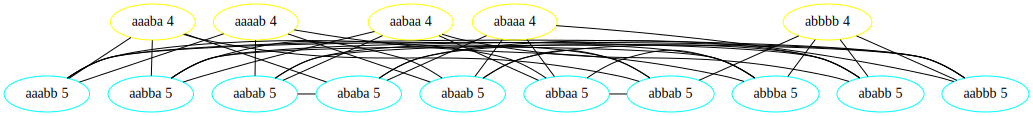
\includegraphics[width=\textwidth]{c_5_2.png}
  \caption{}
  \label{fig:catColorGrouping}
\end{figure}

\pagebreak
\section{Modifications to the existing algorithm}
By not visiting coloring that are equivalent we know this algorithm runs at least as fast original proposed algorithm.

\subsection{Pseudocode}
\begin{verbatim}
DetNRC(H):
  foreach top_coloring(c, F) do
    if DetLocalSearch(H, c, F) then
      return YES
  return NO

DetLocalSearch(H, c, F):
  -- This is the secret sauce
  if g = 0 and induces_raindbow_edge(c, H) then return NO
  if induces_raindbow_edge(c, H).issubset(F) then return NO
  if is_no_rainbow_coloring(c, H) then return YES
  if |e intersect F| != r - 1 forall e in E then return YES
  e' = pick_any(e where |e intersect F| == r - 1)
  v = pick_any(v in (e' - F))
  foreach j in [r] - {c(v)} do
    c' := c but c(v) = j
    if not isSameCategory(c', c) then continue
    if not isRepresentativeColoring(c') then continue
    if DetLocalSearch(H, c', F union {v}) then return YES

  return NO
\end{verbatim}
\pagebreak

\subsection{Proofs}
I am starting to doubt this algorithms correctness.

\subsubsection{All equivalence classes are within the edit distance of $n - r$ from their corresponding \textit{top-node}}
Pick a random surjective coloring $X$. We can now send it to it's representative by renaming the colors, calling the new color $X'$.
We know $X'$ matches the \textbf{eq-regex}, since it is surjective and a representation.

If we now change all but the first appearance of each color to the $a$-color, we have something that matches a \textit{top-node}.
We have $r$ unique colors to pick from, and $n$ nodes.
This means the edit distance from any surjective coloring to its corresponding \textit{top-node} is at most $n - r$. $r$ is the number of frozen nodes.

\subsubsection{Some clarification and an example}
Since the first appearance of a color in the coloring tuple has to be the same -- we can at most replace all other colors.
Consider $aabbcc$, the corresponding \textit{top-node} is $aabaca$.

\subsubsection{We know we visit all coloring categories} 
Since each category (e.g. $(1, 2, 3, 4)$) corresponds to one \textit{top-node} (e.g. $abacaadaaa$) and we visit all \textit{top-nodes} we visit all categories.

\subsubsection{We know we visit all colorings in a coloring category} 
Consider a representative coloring $X$. We know the algorithm only searches within one category at a time, so we can only visit $X$ if we started in the category of $X$.
We know $X$ is reachable from the \textit{top-node} since the frozen nodes of the top-coloring are shared. We can then edit out way closer to $X$ from the \textit{top-node} by visiting other nodes which also have to be part of the same category.

\subsection{Runtime}
Faster, cuts out a large ''chunk'' of the nodes so asymptotically faster -- I really struggle with this. I is somehow related to sterling numbers of the second kind, 
but there's still overlap in the search. But a limitation of the total number of possible states should result in a large speedup.
Maybe a good estimate is $O^*(\left(r-1\right)^{\left(\frac{n\left(r-1\right)}{2r}\right)})$ if I claim I limit the number of coloring by at least a factor 2.


%%%%%%%%%%%%%%%%%%%%%%

\section{A new worst-case optimized algorithm}
This algorithm goes through each equivalent coloring checking if it is a no-rainbow coloring.

\pagebreak
\subsection{Some ''pseudocode''}
The core idea is to just list all equivalence classes and try them. This is the best algorithm that doesn't reason about the edges, since this is the fastest we can test each potential coloring. To make this faster we would need to cut out more colorings that cannot hold.

\begin{adjustbox}{max size={\textwidth}{\textheight}}
\lstinputlisting[language=Python]{no-rainbow-algorithm.py}
\end{adjustbox}

\subsection{Proofs}
The proofs to show this algorithm works as expected.

\subsubsection{All nodes in a category are visited}
Consider a coloring $X$. We can find the top-node by finding the category $C$ this node belongs to.
We try all combinations of colorings.

\subsubsection{Correctness}
We visit all equivalence classes. Since equivalence classes are equivalent in their validity of the coloring we know we've tested all colorings. This program exhaustively tests all colorings, so is correct.

\subsubsection{We visit each coloring exactly once}
(Checked by running the program for $r<10$ and $n < 15$)
TBA

\subsection{Runtime}
Since we can check if the coloring is no-rainbow in polynomial time, and we only visit each equivalence class node once. We can deduce the runtime to $O(S(n, r)/r!)$. Using an estimate (curtsy of Wikipedia), the estimated asymptotic time complexity is $O(\frac{r^n}{r!^2})$ (assuming $r$ is small and $n$ is large).

This is faster for $r > 6$, by quite a wide margin.

\end{document}
